\section{Список определений}
\begin{samepage}
\subsection{Деление целых чисел с остатком.}
Говорят, что целое число $a$ делится на целое число $b$ ($a$ кратно $b$), если $a = bk$ для некоторого целого числа $k$. Разделить целое $a$ на целое положительное $b$ означает найти такое целое $q$ (частное) и такое целое $r$ (остаток), что
\[
a = b \cdot q + r;
\quad
0 \leqslant r < b
\]


\subsection{Сравнения по модулю. Основные свойства.}
Если два числа $a$ и $b$ дают одинаковые остатки при делении на положительное число $N$, то говорят, что они \textit{сравнимы} по модулю $N$, и пишут $a \equiv b \mod{N}$. Сравнение по модулю -- \textit{отношение эквивалентности} на множестве целых чисел.
% \newline
% Основные свойства:
% \begin{enumerate}
%     \item $a + b = b + a$ (коммутативность сложения)
%     \item $a + (b + c) = (a + b) + c$ (ассоциативность сложения)
%     \item $ab = ba$ (коммутативность умножения)
%     \item $a(bc) = (ab)c$ (ассоциативность умножения)
%     \item $a(b + c) = ab + ac$ (дистрибутивность)
%     \item $0+a = a$
%     \item $1 \cdot a = a$
%     \item $0 \cdot a = 0$
% \end{enumerate}
\subsection{Арифметика остатков (вычетов). Обратимые остатки (вычеты).} 
Основные свойства:
\begin{enumerate}
    \item $a + b \equiv b + a$ (коммутативность сложения)
    \item $a + (b + c) \equiv (a + b) + c$ (ассоциативность сложения)
    \item $ab \equiv ba$ (коммутативность умножения)
    \item $a(bc) \equiv (ab)c$ (ассоциативность умножения)
    \item $a(b + c) \equiv ab + ac$ (дистрибутивность)
    \item $0+a \equiv a$
    \item $1 \cdot a \equiv a$
    \item $0 \cdot a \equiv 0$
\end{enumerate}
Остаток (вычет) по модулю $N$ называется \textit{обратимым}, если в произведении с каким-то другим остатком он дает 1. Другими словами, $a$ обратим, если уравнение $ax = 1$  имеет решение.
\end{samepage}
\subsection{Малая теорема Ферма.}
Если $p$ -- простое число и $a$ не делится на $p$, то $a^{p-1}$ сравнимо с $1$ по модулю $p$, то есть $a^{p-1} \equiv 1 \mod{p}$.


\subsection{Функция Эйлера. Теорема Эйлера.}
\textbf{Определение функции Эйлера} \newline
Пусть $N > 1$ -- произвольное целое число, тогда функцию $\varphi(N)$, равную количеству остатков среди $0,1,...,N-1$, взаимно простых с $N$, называют функцией Эйлера.
\newline
Основные свойства функции Эйлера:
\begin{itemize}
    \item $\varphi(p^n) = p^n(1-1/p) = p^{n-1}(p - 1)$ для простого $p$
    \item $\varphi(uv) = \varphi(u)\varphi(v)$, если $u$ и $v$ взаимно просты
\end{itemize}
\textbf{Теорема Эйлера} \newline
Если $a$ и $m$ взаимно просты, то $a^{\varphi(m)} \equiv 1 \mod{m}$, где $\varphi(m)$ -- функция Эйлера.

\subsection{Наибольший общий делитель. Алгоритм Евклида.}
\[
\text{НОД}(a, b) := max (\{ x \> | \> a \text{ кратно } x \} \cap \{ x \> | \> b \text{ кратно } x \})
\]

\begin{lstlisting}[language=Python]
def gcd(a, b):
    if a*b == 0:
        return a + b
    if a > b:
        return gcd(a % b, b)
    return gcd(a, b % a)
\end{lstlisting}




\subsection{\textcolor{orange}{(UNCHECKED)} Расширенный алгоритм Евклида нахождения решения линейного диофантова уравнения.}
\textit{Линейные диофантовы уравнения} -- уравнения вида
\[
a_1x_1 + a_2x_2 + ... + a_nx_n = d,
\] где $a_1,...,a_n$ -- целые числа, а переменные $x_i$ принимают целые значения.
\newline
\newline
Расширенный алгоритм Евклида позволяет находить решения линейного диофантова уравнения 
\[
ax + by = c \text{, где } c = \text{НОД}(a,b).
\]
\begin{lstlisting}[language=Python]
def gcd_expanded(a, b):
    x, x2, y, y2 = 1, 0, 0, 1
    while (a*x + b*y)*(a*x2 + b*y2) > 0:
        if (a*x + b*y) > (a*x2 + b*y2):
            x -= x2
            y -= y2
        else:
            x2 -= x
            y2 -= y
    return (x, y)
\end{lstlisting}




\subsection{Простые числа, формулировка основной теоремы арифметики.}
Целое число $p > 1$ называется \textit{простым}, если оно не разлагается в произведение меньших чисел (то есть не имеет положительных делителей, кроме 1 и $p$).
\newline
\newline
Всякое целое положительное число, большее 1, разлагается на простые множители, причем единственным образом: любые два разложения отличаются только перестановкой сомножителей.



\subsection{Равномощные множества.}
Множество $A$ называется равномощным множеству $B$, если существует биекция из множества $A$ в множество $B$.
\newline
Свойства равномощности:
\begin{itemize}
    \item \textit{Отношение равномощности симметрично}: если $A$ равномощно множеству $B$, то $B$ равномощно $A$. В самом деле, как мы уже обсуждали, ко всякой биекции есть обратная функция — тоже биекция.
    \item \textit{Отношение равномощности рефлексивно}: каждое множество равномощно само- му себе. В самом деле, тождественная функция, которая отображает каждый элемент какого-то множества $A$ в себя, является биекцией между $A$ и $A$.
    \item \textit{Отношение равномощности транзитивно}: если $A$ равномощно $B$ и $B$ равномощно $C$, то $A$ равномощно $C$, так как композиция биекций -- биекция.
\end{itemize}
Таким образом, отношение равномощности является \textit{отношением эквивалентности}.


\subsection{Счётные множества.}
Счётные множества -- это множества равномощные множеству натуральных чисел $\mathbb{N}$.
\newline
Основные свойства счётных множеств:
\begin{itemize}
    \item \textit{Объединение двух счётных множеств счётно.}
    \item \textit{Всякое подмножество счётного множества конечно или счётно.}
    \item \textit{Всякое бесконечное множество содержит счётное подмножество.}
    \item \textit{Множество рациональных чисел $\mathbb{Q}$ счетно.}
    \item \textit{Объединение конечного или счётного числа конечных или счётных множеств конечно или счётно.}
    \item \textit{Декартово произведение двух счетных множеств $A \times B$ счетно.}
\end{itemize}


\subsection{Множества мощности континуум.}
Множество $A$ имеет мощность континуум, если $A$ равномощно $\mathbb{R}$.
\newline
Основные свойства:
\begin{itemize}
    \item  $[0,1] \sim \mathbb{R}$
    \item  $(0,1) \sim \mathbb{R}$
    \item  $\mathbb{R} \times \mathbb{R} \sim \mathbb{R}$
    \item Множество бесконечных последовательностей нулей и единиц несчётно.
    \item Отрезок $[0, 1]$ равномощен множеству бесконечных последовательностей из нулей и единиц.
\end{itemize}

\subsection{Основные определения элементарной теории вероятностей: исходы, события, вероятность события.}
\textit{Вероятностным пространством} называется конечное множество $U$, которое состоит из \textit{возможных исходов} и на котором задана функция $Pr : U \to [0, 1]$, такая что $\sum_{ x \in U} Pr(x) = 1$.
\newline
\newline
Функция $Pr$ называется \textit{вероятностным распределением}, а число $Pr(x)$ называется \textit{вероятностью исхода} $x \in U$.
\newline
\newline
\textit{Событием} называется произвольное подмножество $A \subset U$, состоящее из \textit{благоприятных исходов}.
\newline
\newline
\textit{Вероятностью события} $A$ называется число $Pr[A] = \sum_{x \in A} Pr(x)$.
\newline
\newline
В \textit{модели с равновозможными исходами} функция $Pr$ задается формулой $Pr[x] = 1/|U|$ для всякого $x \in U$ (такое распределение называют также \textit{равномерным}). Тогда вероятность события $A$ равна $Pr[A] = |A|/|U|$.



\subsection{Формулировка формулы включений и исключений для вероятностей.}
Если $A, B \subset U$, то 
\(
Pr[A \cup B] = Pr[A] + Pr[B] - Pr[A \cap B].
\)
В частности, \(
Pr[A \cup B] \leqslant Pr[A] + Pr[B]
\) и, если $Pr[A \cap B] = 0$, то \(
Pr[A \cup B]=Pr[A]+Pr[B].
\)
\newline
\newline
Для любых $A_1, ... , A_n \subset U$ верно
\[
Pr [
\bigcup_{i=1}^n A_i
] \leqslant
\sum_{i=1}^n Pr[A_i],
\]
а если множества $A_i$ попарно не пересекаются, то неравенство обращается в равенство (это называется аддитивностью вероятностей для попарно несовместных событий).
\newline
\newline
В \textit{равновозможной модели} для произвольных множеств $A_1,...,A_n \subset U$ верно
\[
Pr[A_1 \cup A_2 \cup ... \cup A_n] = \sum_i Pr[A_i] - \sum_{i<j} Pr[A_i \cap A_j] + ... = \sum_{\varnothing \neq I \subset \{1,2,...,n\}} (-1)^{|I| + 1} Pr \left[ \bigcap_{i \in I} A_i \right].
\]


\subsection{Условная вероятность.}
\textit{Условной вероятностью события $A$ при условии $B$} называется число
\[
Pr[A | B] = \frac{Pr[A \cap B]}{Pr[B]}.
\]
\begin{lemma}
\normalfont{(формула Байеса).} Если вероятность событий $A$ и $B$ положительна, то
\[
Pr[A | B] = Pr[A] \cdot \frac{Pr[B | A]}{Pr[B]}.
\]
\end{lemma}


\subsection{Независимые события. Основные свойства независимых событий.}
События $A$ и $B$ называются независимыми, если $Pr[A | B] = Pr[A]$ при $Pr[B] > 0$. 
\newline
Основные свойства независимых событий:
\begin{itemize}
    \item Если события $A$ и $B$ независимы, то события $A$ и $\overline{B}$, $\overline{A}$ и $B$, $\overline{A}$ и $\overline{B}$ также независимы.
    \item Если события $A$ и $B$ независимы, то $Pr[AB] = Pr[A] \cdot Pr[B]$.
\end{itemize}


\subsection{Формула полной вероятности.}
Пусть $B_1,...,B_n$ -- разбиение вероятностного пространства U, то есть $U = B_1 \cup ... \cup B_n$, где $B_i \cap B_j = \varnothing$ при $i \neq j$. Пусть также $Pr[B_i] > 0$ для всякого $i$. Тогда для всякого события $A \subset U$
\[
Pr[A] = \sum_{i=1}^n Pr[A | B_i] \cdot Pr[B_i].
\]




\subsection{Случайная величина и математическое ожидание. Линейность математического ожидания.}
\textit{Случайная величина} -- это числовая функция на вероятностном пространстве, то есть функция вида $f : U \to \mathbb{R}$.
\newline
\newline
\textit{Математическим ожиданием} случайной величины $f : U \to \mathbb{R}$ называется число
\[
E[f] = \sum_{u \in U} f(u)Pr(u)
\]
\newline
Пусть $f : U \to \mathbb{R}$ и $g : U \to \mathbb{R}$ -- две случайные величины на одном и том же вероятностном пространстве. Тогда
\[
E[f + g] = E[f] + E[g]. 
\]



\subsection{Формулировка неравенства Маркова.}
Пусть $f$ — случайная величина, принимающая только неотрицательные значения. Тогда для всякого $\alpha > 0$ верно
\[
Pr[f \geqslant \alpha] \leqslant \frac{E[f]}{\alpha}.
\]

\subsection{Определение схемы в некотором функциональном базисе. Представление схем графами.}
\begin{wrapfigure}{r}{0.4\textwidth}
    \centering
    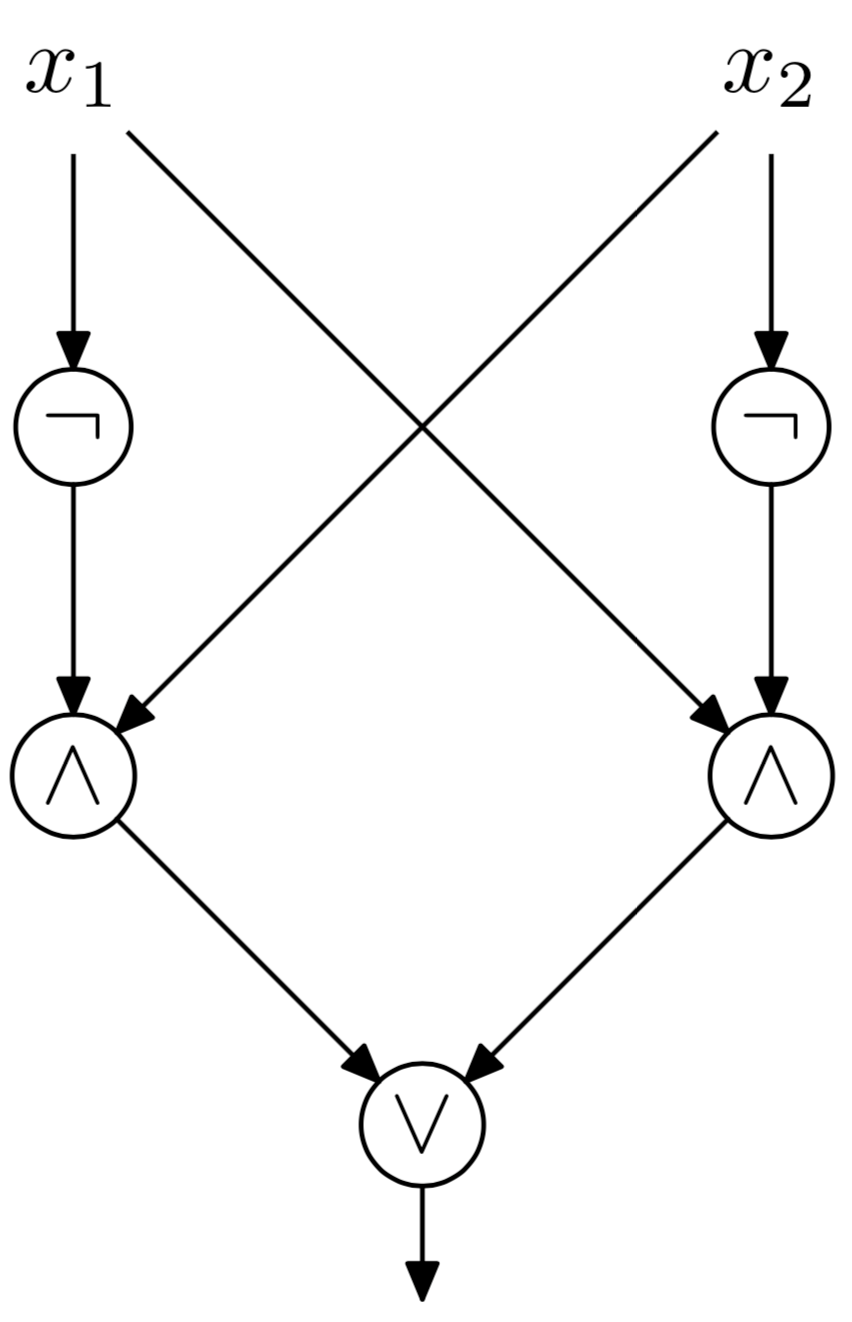
\includegraphics[width=0.25\textwidth]{graph}
    \caption{Схема для функции $x_1 \oplus x_2$}
\end{wrapfigure}

\textit{Булевой схемой} от переменных $x_1, ..., x_n$ называется последовательность булевых функций $g_1,...,g_s$, в которой всякая $g_i$ получается из предыдущих функций последовательности и переменных применением одной из логических операций: отрицание, конъюнкция и дизъюнкция. Другими словами, для всякого $i$ имеет место одно из равенств
\[
g_i = g_j \wedge g_k \> (j, k < i),
\quad
g_i = g_j \vee g_k \> (j,k < i),
\]
\[
g_i = g_j \wedge x_k \> (j < i),
\quad
g_i = g_j \vee x_k \> (j < i),
\]
\[
g_i = x_j \wedge x_k,
\quad
g_i = x_j \vee x_k,
\]
\[
g_i = \neg g_j \> (j < i),
\quad
g_i = \neg x_k.
\]
Имея в виду эти связи между элементами последовательности (схемы), будем также называть элементы схемы \textit{присваиваниями}.
\newpage

\subsection{Полный базис. Примеры полных и неполных базисов.}
\textit{Полный логический базис} -- это такая система логических функций, с помощью которых можно записать любую, сколь угодно сложную функцию. 
\newline
Примеры полных логических базисов:
\begin{itemize}
    \item $\{\wedge, \vee, \neg\}$
    \item $\{\vee, \neg\}$
    \item $\{\wedge, \neg\}$
    \item $\{x \downarrow y\}$ (стрелка Пирса)
    \item $\{x | y\}$ (штрих Шеффера)
    \item $\{\wedge, \oplus, 1 \}$ (базис Жегалкина)
\end{itemize}
Примеры неполных логических базисов:
\begin{itemize}
    \item $\{\wedge, \vee\}$
    \item $\{\oplus \}$
\end{itemize}




\subsection{Полином Жегалкина (в стандартном виде).}
Выражения вида
\[
P(x_1,...,x_n) = a_0 \oplus a_1x_1 \oplus a_2x_2 \oplus ... \oplus a_nx_n \oplus a_{12}x_1x_2 \oplus a_{13}x_1x_3 \oplus ... \oplus a_{1...n}x_1...x_n,
\quad
a_0,...,a_{1...n} \in \{0,1\}.
\]
называются \textit{полиномами Жегалкина}.
\newline
\newline
Всякая булева функция представима в виде полинома Жегалкина и притом единственным образом.


\subsection{Схемная сложность функции (размер схемы).}
\textit{Схемная сложность} булева отображения $f : \{0, 1\}^n \to \{0, 1\}^m$ (в частности, булевой функции) — это наименьший размер схемы, вычисляющей это отображение.
\newline
\newline
Всякую функцию $f : \{0, 1\}^n \to \{0, 1\}$ можно вычислить схемой размера не больше $O(n2^n)$.




\newpage


\section{\textcolor{red}{(TODO)} Примерные задачи на понимание материала курса}
 
\subsection*{\normalsize{\normalfont{
Привидите пример таких целых чисел $a, b, c$, что НОД$(ab,c) \neq $НОД$(a,c) \cdot $НОД(b,c).
}}} 